\chapter{倉庫でHuman-in-the-loopした場合のシミュレーション検証}

第\ref{chap:method}章で紹介した2通りの方法を用いて,人間が必要とされる具体的な事例をいくつか想定し,それらの方法を用いて問題解決できることを示す.2台のロボットと1人の人間についてスーパーバイザ制御を行い,計算されたスーパーバイザをもとにシミュレーションを作成する.ロボット1とロボット2のオートマトンをそれぞれ$G_1,G_2$とかき,人間のオートマトンを$H$とかく.

\section{ケース1:棚から商品が落下した場合} \label{sect:case1}
%本研究では,スーパーバイザの計算結果から,最適なふるまいを選び出す.
%全エージェントを同時に動いたとする.
%人間の安全を保障するため,最後に人間の行動を決定する.
%

1つ目のケースでは,人間の臨機応変な対処ができる能力を駆使し,発生の予測が不可能かつ早急に措置しなければならないトラブルに対処することが目的である.

まず,商品が棚から落ちた図\ref{fig:HITL1_case1}のような場合を初期状態と考える.2台のロボットの初期状態は計算上,0としているが,ロボット1($blue$)は状態7の上に,ロボット2($green$)は状態8の上に,一方人間の初期状態である通常作業場所は状態67の下に位置している.またそれぞれのタスクについて,ロボット1は状態33(棚)に,ロボット2は状態36(棚)に,人間はトラブルの発生した場所である状態26(通路上)に設定する.搬出場所については計算上71とするが,$G_1$は状態68の下に,$G_2$は状態65の下に,人間$H$はもとの作業場所であった状態67の下に戻ることとする.

\begin{figure}[t]
    \centering
    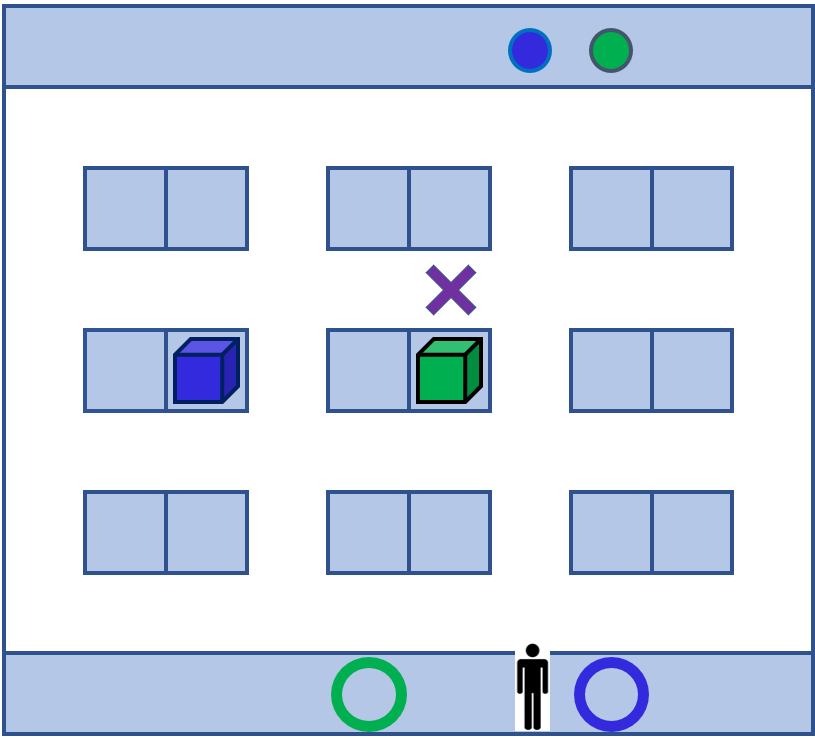
\includegraphics[scale=0.25]{figures/HITL1_case1.png}
    \caption{初期状態(ケース1)}
    \label{fig:HITL1_case1}
\end{figure}

ケース1では,人間は棚から落ちた商品をもとあった収納スペースに返し,すぐ元の作業場所へ戻ってくると想定する.

ロボットのオートマトン$G_1$,$G_2$と人間のオートマトン$H$の遷移関数はそれぞれの最短経路のみで定義するので,経路はそれぞれ図\ref{fig:HITL1_case1_G1},\ref{fig:HITL1_case1_G2},\ref{fig:HITL1_case1_H}とする.

\begin{figure}[b]
    \centering
    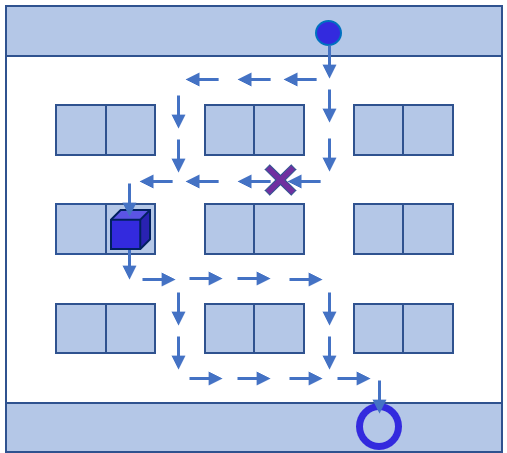
\includegraphics[scale=0.38]{figures/HITL1_case1_G1.png}
    \caption{ロボット1の経路(ケース1)}
    \label{fig:HITL1_case1_G1}
\end{figure}
\begin{figure}[!t]
    \centering
    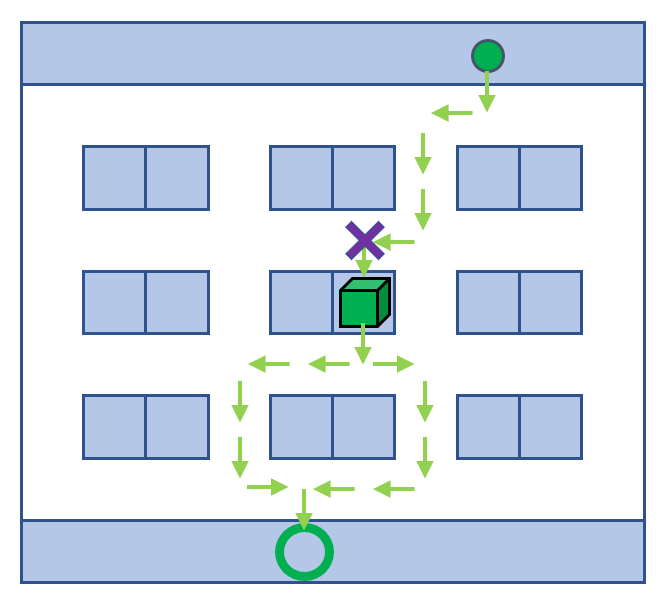
\includegraphics[scale=0.3]{figures/HITL1_case1_G2.png}
    \caption{ロボット2の経路(ケース1)}
    \label{fig:HITL1_case1_G2}
\end{figure}
\begin{figure}[!t]
    \centering
    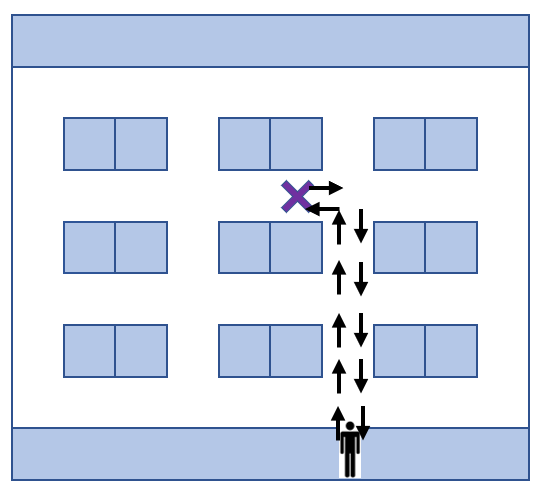
\includegraphics[scale=0.35]{figures/HITL1_case1_H.png}
    \caption{人間の経路(ケース1)}
    \label{fig:HITL1_case1_H}
\end{figure}

落ちた商品で通路を塞いでしまうのでそのことに関しても考慮しなければならない.

このケースは,ロボット1ではトラブルの発生場所である状態26を通る経路がいくつかある最短経路のうちの1つとなっている.ロボット1に関して言えば,落下した商品で通路が使用できなくなっている経路を削除しても支障はない.しかし,ロボット2のオートマトン$G_2$のようにトラブルの発生場所を使う経路しか定義されていないとき,そもそも受理状態まで到達できないという問題点が挙げられる.また,仮に搬出場所付近でこのトラブルが発生したとき,トラブルが処理されてすでに通ることができるにもかかわらず経路を削除してしまい効率の良いふるまいを見逃す可能性もある.
落下した商品に関するオートマトンを作成し,それをもちいて制御要求を定めることで,これらの問題を解決する.

%通路に落ちた商品で経路を塞いでしまう問題を解決する.
商品に関するオートマトン$O$は通路に落ちている状態0と棚に収納されている状態1の2つの状態で構成されるオートマトンで,初期状態を0,受理状態を1とする(図\ref{fig:automatonO}).状態遷移は人間がトラブルを処理する事象(人間と共通の事象)が発生したとき,0から1に移る状態遷移のみ定義する.ここで,指定した状態の組を排除するmutexという関数をもちいて制御要求を定める.

$G_1$と$O$,$G_2$と$O$について,mutexを使用し,状態の組み合わせ$P_{O,G_i}=[0,26]$を取り除く制御要求を与える. $P_{O,G_i}$の1つ目の要素は$O$の状態,2つ目の要素は$G_i$の状態を示している.こうしてロボットの状態とトラブルが処理できていない状態の組み合わせを除くことで,商品が通路上にあるとき塞がった通路の使用を禁止し,かつ商品が棚に戻されたあとは通路の使用を許可する制御要求を与える. 

\begin{figure}[t]
    \centering
    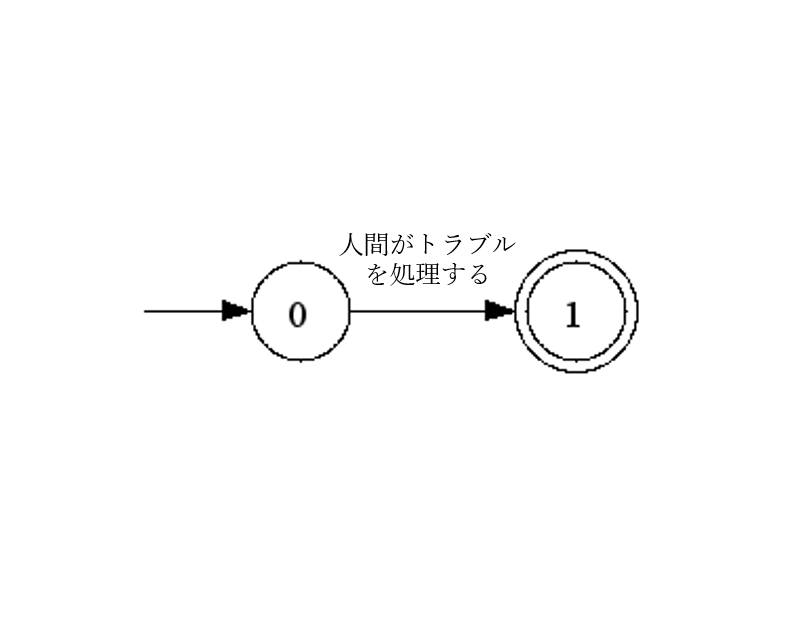
\includegraphics[scale=0.4]{figures/automatonO.png}
    \caption{落下した商品についてのオートマトン}
    \label{fig:automatonO}
\end{figure}

$H$の状態遷移の定義について,スタート地点からトラブルが発生した場所へ向かう遷移と,その逆にトラブルの場所からもといた場所へ戻ってくる遷移があり,方法1では,これらはすべて不可制御事象によって遷移する.極端な話,1マス進んで1マス戻るという遷移で受理状態に到達する可能性もあるが,スーパーバイザは行動を禁止することができずこれに対して対処できない.トラブルの発生場所を通る経路しか定義されていないロボットが含まれていた場合,人間のトラブル処理の事象が起こるまで受理状態にいくことはない.しかし,先ほどの1マス進んで1マス戻る例では,人間がトラブルを処理せず受理状態に到達する可能性があるため,条件を満たすスーパーバイザが存在しないことになる.

\begin{figure}[!t]
    \centering
    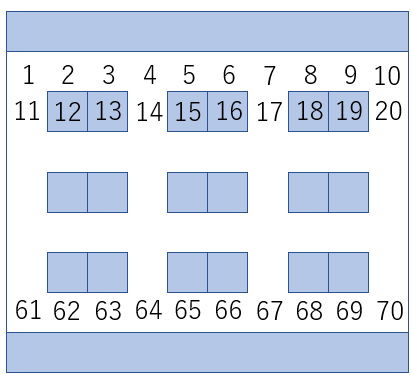
\includegraphics[scale=0.5]{figures/Warehouse_before.png}
    \caption{トラブルの処理前の状態に割り当てる番号}
    \label{fig:Warehouse_before}
\end{figure}
\begin{figure}[!t]
    \centering
    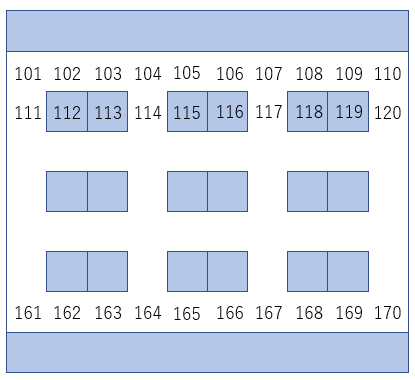
\includegraphics[scale=0.5]{figures/Warehouse_after.png}
    \caption{トラブルの処理後に状態に割り当てる番号}
    \label{fig:Warehouse_after}
\end{figure}

人間の遷移が可制御事象で定義されていれば,オートマトン$O$を制御要求にすることにより,人間がトラブルを処理する前に受理状態に到達することがないように設定が可能だ.しかし,人間の行動を不可制御事象にしてこの制御要求を与えても,条件を満たすスーパーバイザは存在しない.

これを解決するため,行きの状態と帰りの状態を区別することで,トラブルを処理する前に途中で引き返して受理状態にたどり着かないように設計した.状態の番号を図\ref{fig:Warehouse_before},\ref{fig:Warehouse_after}のように割り当てる.トラブルを処理する事象が起これば,帰り用の状態に遷移する.

商品で通路が塞がれているときはその場所を通る経路を削除し,人間がトラブルを処理したのち,削除した経路を追加しスーパーバイザの再計算を行うという方法も考えたが,現時点ではオンライン制御を実現できておらず,今後の課題として検討する.

\subsection{方法1} \label{sec:case1_method1}
方法1の場合,人間の行動を表\ref{tb:event_numbers_human1}のように定義することで,人間の経路はロボットからみてすべて通行不可となる方法であった.ここで,北,東,南,西に進む事象は,図で示すとそれぞれ上,右,下,左に進むことを意味する.トラブルを処理する事象は状態$s$に存在したとすると,状態$s$から状態$s+100$に遷移するという事象である.ロボットの進入禁止エリアは図\ref{fig:human_area}のように表され,人間が通る可能性がある限りロボットは進入できない.

\begin{table}[htb]
    \centering
    \begin{tabular}{|c|c|} \hline
        事象 & 番号 \\ \hline
        北へ進む & $100$ \\
        東へ進む & $102$ \\
        南へ進む & $104$ \\
        西へ進む & $106$ \\ 
        トラブルを処理する & $108$ \\ \hline
    \end{tabular}
    \caption{$H$の事象に振られる番号(ケース1,方法1)}
    \label{tb:event_numbers_human1}
\end{table}

\begin{figure}[!t]
    \centering
    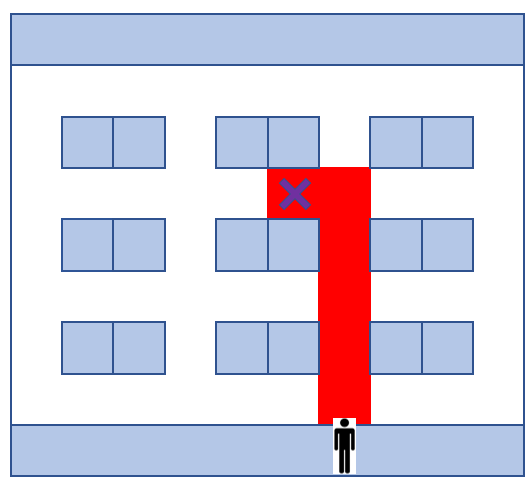
\includegraphics[scale=0.3]{figures/5_human_area.png}
    \caption{ロボットの進入禁止エリア(ケース1,方法1)}
    \label{fig:human_area}
\end{figure}

行きと帰りの状態を分けることで起こってしまう問題がある.それは,トラブルを処理した後で,人間が通り過ぎたところからロボットが通路として使用するのが許可されることだ.作業場所に戻っている最中の人間のすぐ後ろをロボットが追尾する行動を許してしまうことになる.これでは,十分に安全ということはできない.

ここで新しいオートマトン$P$を定義する.図\ref{fig:automatonO}のオートマトンのように,状態が2つ,遷移関数は初期状態から受理状態に遷移する事象ただ1つのみで定義する.$H$が受理状態にいるときに自己ループする事象を定義し,その事象と$P$の唯一の事象を一致させることによって,$H$が受理状態に到達した後で,$P$は状態0から状態1に遷移することになる.

そして,mutexを使用し,$P$が状態0に,$G_1,G_2$が人間の経路上の状態に存在する組み合わせを排除する.
これを制御要求に追加することで人間がもともといた作業場所に戻るまで,人間の経路に侵入するロボットの行動を禁止し続けることが可能である.
オートマトン$P$は,人間が搬出場所に戻ったときのみ作動する,人間の安全を確認するスイッチのような働きをする.

$G_1,G_2$と$H$について,衝突が起こらないようにそれぞれが同じ状態にいる状態を$PLANT$から除く要求と,通路に落ちた商品が棚に戻されるまで,落ちた商品の位置にいる状態を除く要求を制御要求として与える.これらの制御要求をもとにスーパーバイザを作成し,フィードバックループ制御システムを構成する.

スーパーバイザによってどのような制御アクションを行われるかシミュレーションで解説する.

図\ref{fig:HITL1_case1_a}のような状態を状態$a$と呼ぶことにする.状態$a$のときロボット1は状態7に位置しており,ロボット2は状態8に位置している.このとき,次に生起するロボットの行動の選択肢として,$G_1$が行動15によって状態17へ遷移,$G_1$が行動17によって状態6へ遷移,$G_2$が行動27により状態7へ遷移する3つが存在する.
ここでロボット2が行動17で左に移動してしまった場合はロボット1と衝突することになり,制御要求を満たさない.そのため,このときスーパーバイザは$G_2$の行動27を禁止する.このとき,その他の遷移はスーパーバイザに制御されることなく生起が許可されている.

\begin{figure}[!t]
    \centering
    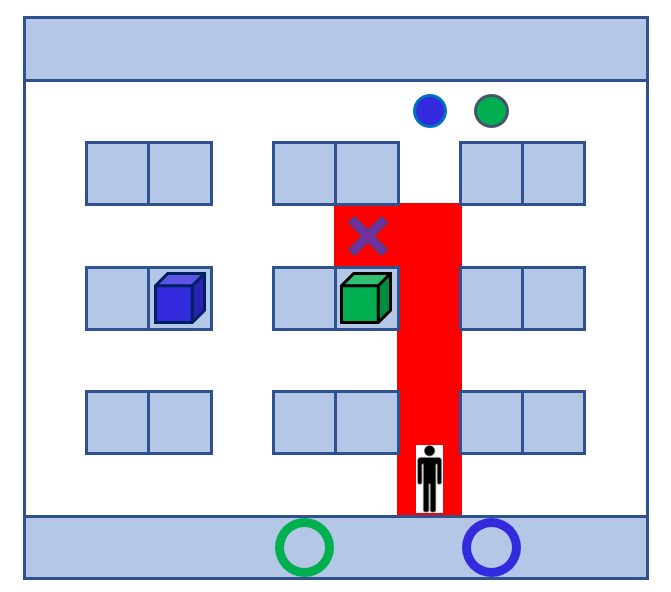
\includegraphics[scale=0.3]{figures/HITL1_case1_a.png}
    \caption{ケース1\ 状態$a$}
    \label{fig:HITL1_case1_a}
\end{figure}

\begin{figure}[!t]
    \centering
    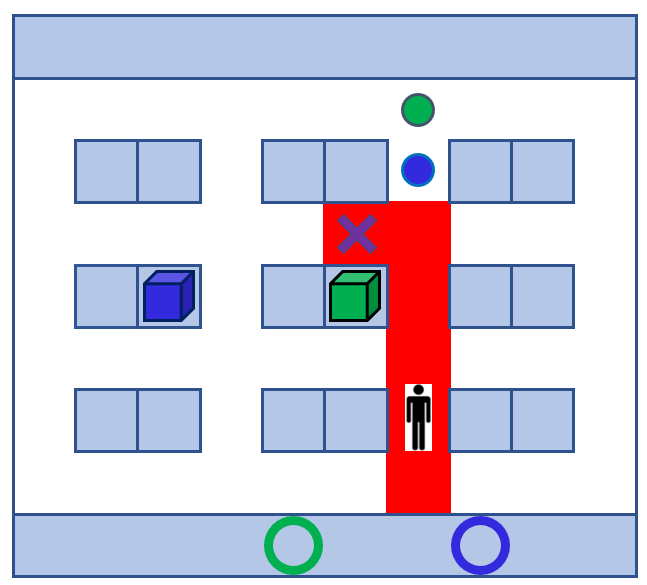
\includegraphics[scale=0.3]{figures/HITL1_case1_b.png}
    \caption{ケース1\ 状態$b$}
    \label{fig:HITL1_case1_b}
\end{figure}

$G_1$は行動15を許可されているので,状態17に進み,その他のエージェント達も遷移して状態$a$から状態$b$(図\ref{fig:HITL1_case1_b})になったと仮定する.このとき状態17からの$G_1$の遷移は行動15により状態27へ移る遷移だけである.しかし,状態27は人間の経路上に指定されているので,スーパーバイザが$G_1$のこの行動を禁止する.人間がトラブルを処理してもとの作業場所に戻るまで,つまり$H$が状態167($G_1$から見ると状態67)から受理状態に遷移して,受理状態での自己ループ事象が生起されるまで,$G_1$の次の行動が禁止され続けることになる.

\begin{figure}[!t]
    \centering
    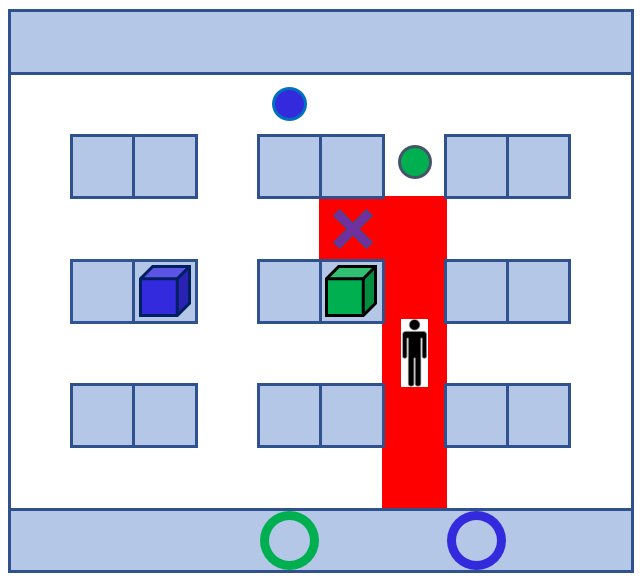
\includegraphics[scale=0.3]{figures/HITL1_case1_c.png}
    \caption{ケース1\ 状態$c$}
    \label{fig:HITL1_case1_c}
\end{figure}

\begin{figure}[!t]
    \centering
    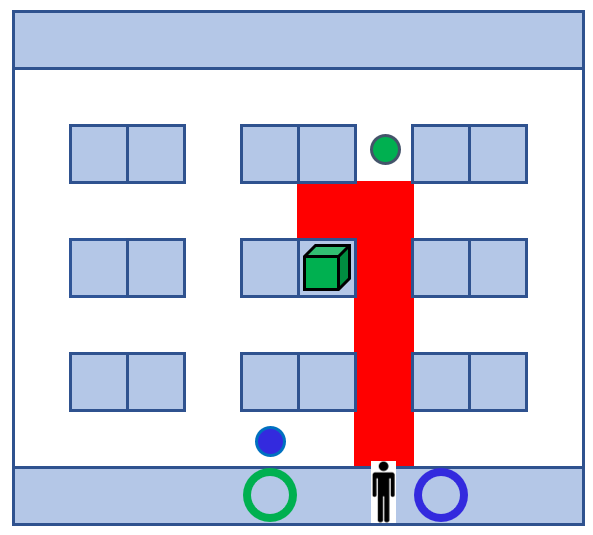
\includegraphics[scale=0.32]{figures/HITL1_case1_d.png}
    \caption{ケース1\ 状態$d$}
    \label{fig:HITL1_case1_d}
\end{figure}

また,状態$a$から,$G_1$が行動17,$G_2$が行動25,$H$が行動100が生起したときの状態を状態$c$(図\ref{fig:HITL1_case1_c})とする.このときも状態$b$のとき同様に,状態17にいる$G_2$の遷移は行動25だけで,行動25により遷移した場合,人間の使用する通路に入ってしまう.制御要求を満たさないので,$H$が受理状態である171で自己ループするまで$G_2$の行動25が禁止される.

%人間がトラブルを処理したのち図\ref{fig:HITL1_case1_d} のように人間が状態37に遷移すると,状態27に人間の通る可能性がなくなり,行動25がスーパーバイザによって許可される.
$H$が受理状態171で安全が確保されたのち,図\ref{fig:HITL1_case1_d}のようにロボットの進入禁止エリアが解除され,対象がロボットだけの自動化制御が行われる.

\begin{figure}[!t]
    \centering
    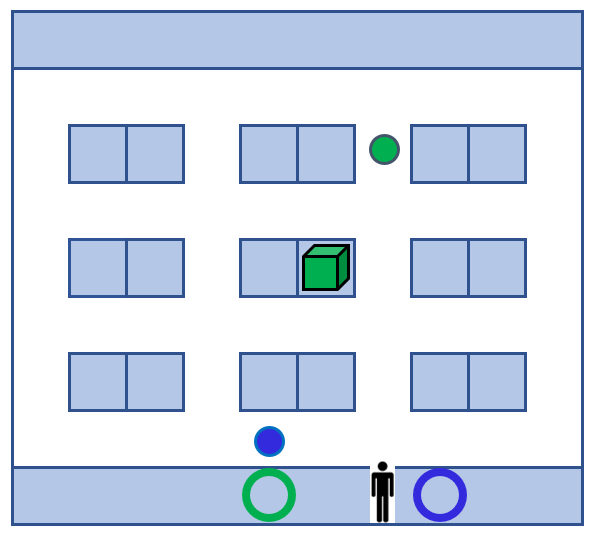
\includegraphics[scale=0.32]{figures/HITL1_case1_e.png}
    \caption{ケース1\ 状態$e$}
    \label{fig:HITL1_case1_e}
\end{figure}



\subsection{方法2}
次に先ほどと同じ例を用いて,方法2によって制御した場合のスーパーバイザについて解説する.

まず,人間の行動を表\ref{tb:event_numbers_human2}のように可制御事象で定義する.

\begin{table}[htb]
    \centering
    \begin{tabular}{|c|c|} \hline
        事象 & 番号 \\ \hline
        北へ進む & $101$ \\
        東へ進む & $103$ \\
        南へ進む & $105$ \\
        西へ進む & $107$ \\ 
        トラブルを処理する & $109$ \\ \hline
    \end{tabular}
    \caption{$H$の事象に振られる番号(ケース1,方法2)}
    \label{tb:event_numbers_human2}
\end{table}

\begin{figure}[!t]
    \centering
    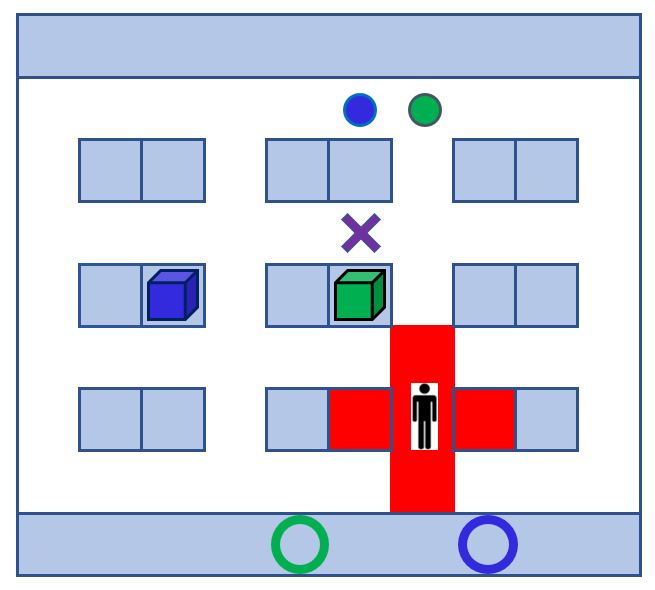
\includegraphics[scale=0.3]{figures/HITL2_case1_f.png}
    \caption{ケース1\ 状態$f$}
    \label{fig:HITL2_case1_f}
\end{figure}

\begin{figure}[!t]
    \centering
    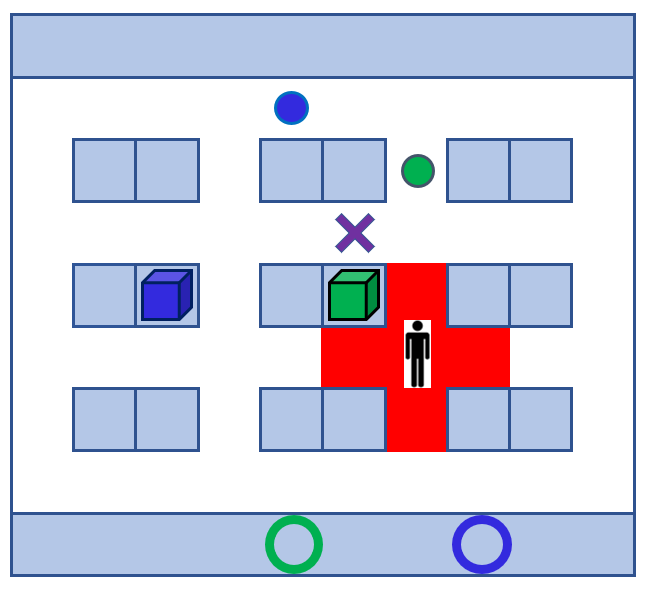
\includegraphics[scale=0.3]{figures/HITL2_case1_g.png}
    \caption{ケース1\ 状態$g$}
    \label{fig:HITL2_case1_g}
\end{figure}

状態$f$(図\ref{fig:HITL2_case1_f})のとき,ロボット2のとり得る遷移は行動25である.しかし,このとき行動25により,状態17に遷移してその他のエージェントも遷移したとき,状態$g$(図\ref{fig:HITL2_case1_g})になる.商品を棚に戻す作業をしない限り,ロボットは状態26に遷移できない制御要求があるのでロボット2は状態27に遷移したとしても受理状態まで到達することはない.また,人間とロボットの間に1マス以上間隔を開けなければいけない制御要求が与えられているため人間は状態27に遷移することができない.この結果,ロボット2と人間はお互い遷移ができないブロッキング状態に陥る.これを防ぐため,スーパーバイザは,状態$f$で,$G_2$の行動25を禁止する.

\begin{figure}[h]
    \centering
    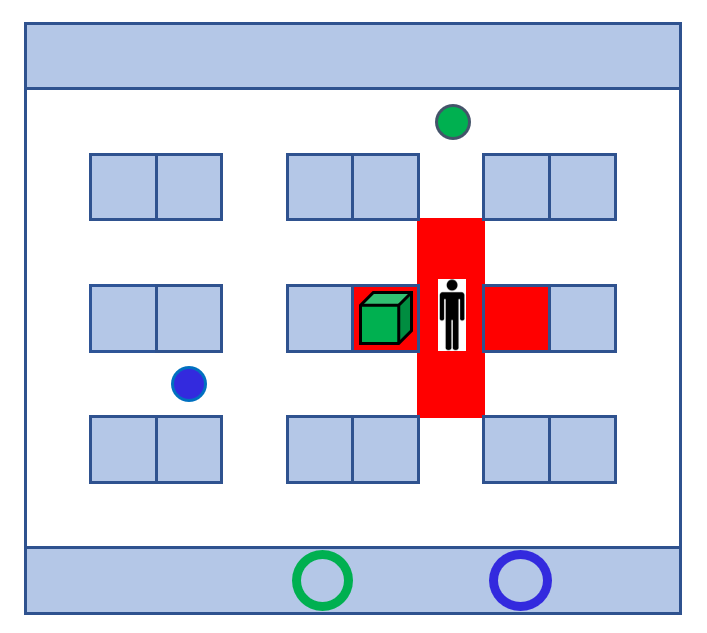
\includegraphics[scale=0.3]{figures/HITL2_case1_h.png}
    \caption{ケース1\ 状態$h$}
    \label{fig:HITL2_case1_h}
\end{figure}

$H$が状態137に遷移した後(図\ref{fig:HITL2_case1_h}),$G_2$の状態7での行動25が許される.


\section{ケース2:人間とロボットが協調する}
% ケース4では,ロボットが荷物を積み込むときに人間の助けが必要な場合
% d=1でいい理由も書く??

段ボール箱単体や,段ボール箱が乗ったパレットを運搬するような単純作業を行う場合,ロボットは能力を発揮する.それに比べて,商品のピッキング作業は不得意であり,今のピッキング技術では,商品の条件に変化があるような複数のタスクを1つのロボットで担うのは,困難であり,近い将来実現するのは難しいと考えられる.また人間は,ピッキング作業を得意としており,小さい品や,柔らかいもの,つぶれやすいものなど,さまざまな商品の条件に対応することができる.

荷物の運搬において,迅速に,かつ一度で大量に運ぶことも可能なロボットと,ピッキング作業において能力を発揮できる人間のそれぞれの長所を生かすことを目的として考えられた事例の制御システムを設計する.

ケース2では,具体的な例として図\ref{fig:HITL1_case2}を考え,ロボットだけでは完遂できない特殊なタスクが状態32(棚)にあり,ロボット1に与えるとする.状態4の上をスタート地点とし,状態64の下に位置する搬出場所へ届けるというタスクが割り当てられている場合を想定する.また,ロボット2にはスタート地点を状態6の上に,搬出場所を状態68の下に,ピックする商品が状態33(棚)にあるタスクを与える.
人間は普段の作業場所を状態66の下とおいて,状態31(通路上)に向かい,ロボット1の手助けをする.このときの人間のポジションを協調作業場所と呼ぶことにする.ケース1と同様に,初期状態と受理状態を普段の作業場とする.

\begin{figure}[!t]
    \centering
    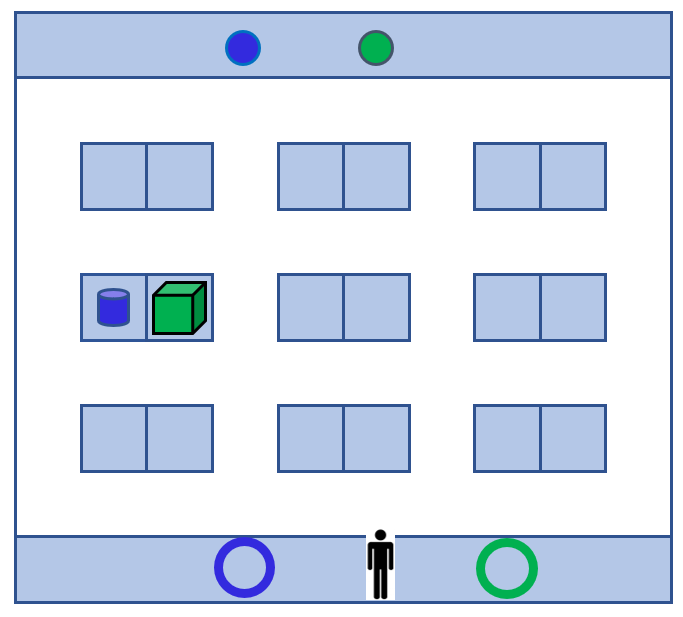
\includegraphics[scale=0.3]{figures/HITL1_case2.png}
    \caption{ケース2\ 初期状態}
    \label{fig:HITL1_case2}
\end{figure}

それぞれの最短経路は図\ref{fig:HITL1_case2_G1},\ref{fig:HITL1_case2_G2},\ref{fig:HITL1_case2_H}になる.

\begin{figure}[!t]
    \centering
    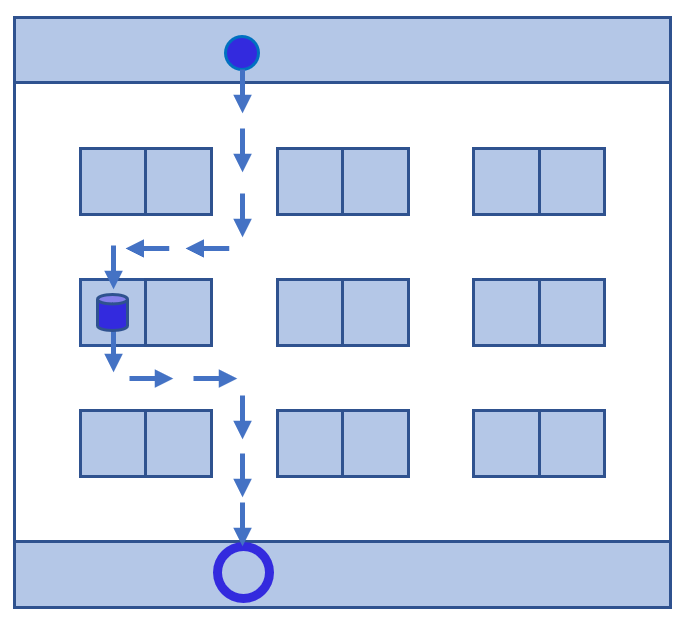
\includegraphics[scale=0.3]{figures/HITL1_case2_G1.png}
    \caption{ロボット1の経路(ケース2)}
    \label{fig:HITL1_case2_G1}
\end{figure}
\begin{figure}[!t]
    \centering
    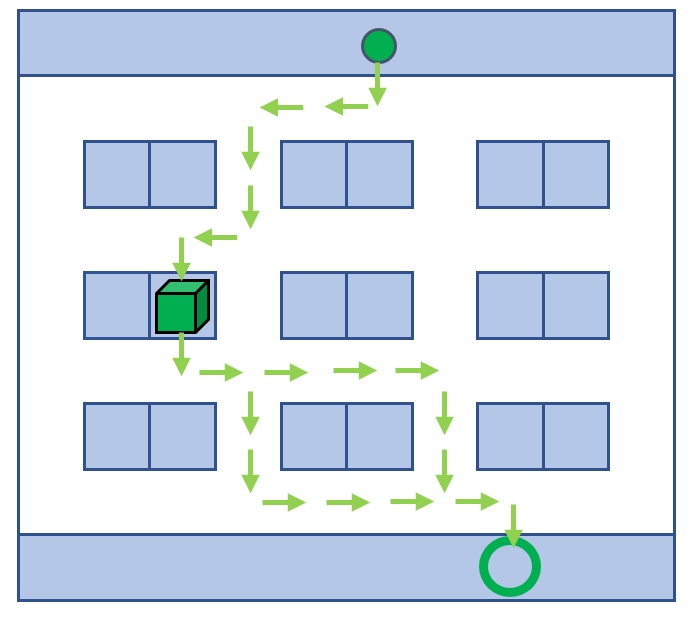
\includegraphics[scale=0.3]{figures/HITL1_case2_G2.png}
    \caption{ロボット2の経路(ケース2)}
    \label{fig:HITL1_case2_G2}
\end{figure}
\begin{figure}[!t]
    \centering
    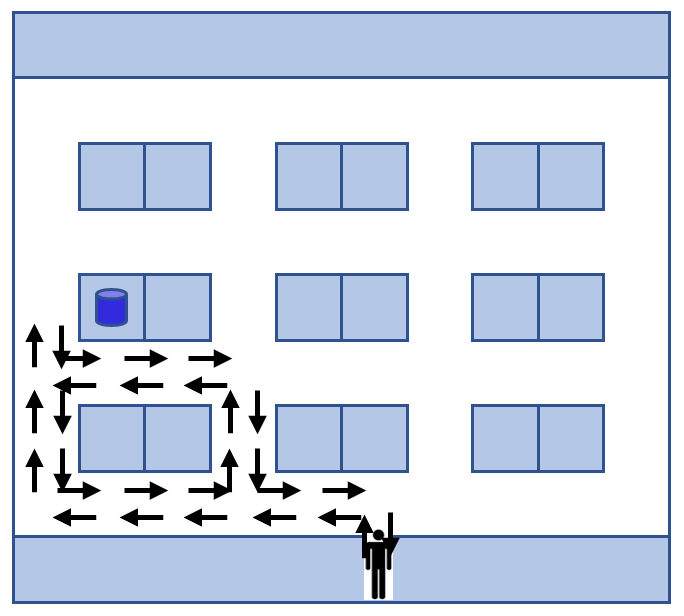
\includegraphics[scale=0.3]{figures/HITL1_case2_H.png}
    \caption{人間の経路(ケース2)}
    \label{fig:HITL1_case2_H}
\end{figure}

またケース1と同様に,図\ref{fig:Warehouse_before},\ref{fig:Warehouse_after}のように行きの状態と帰りの状態を分ける必要がある.


\subsection{方法1}
まず,人間の事象を表\ref{tb:event_numbers_human3}のように設定し,オートマトン$H$を作成する.またロボットの進入禁止エリアは図\ref{fig:human_area_2}となる.

\begin{figure}[!t]
    \centering
    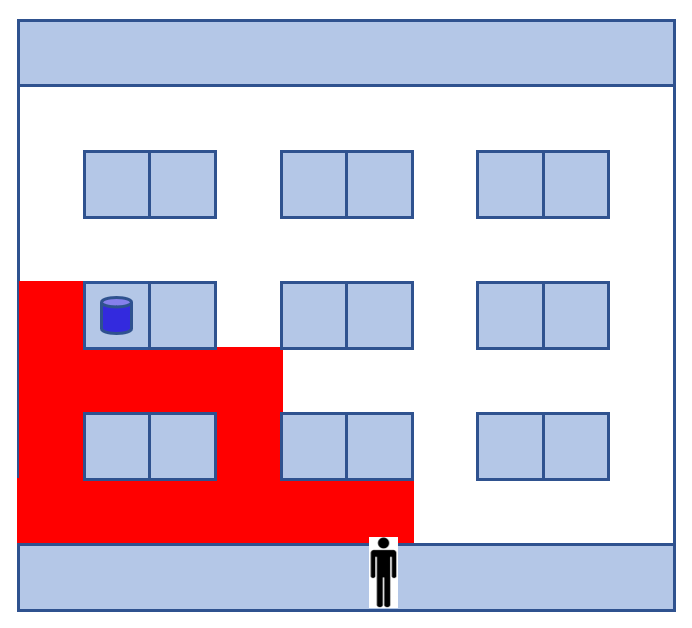
\includegraphics[scale=0.3]{figures/human_area_2.png}
    \caption{ロボットの進入禁止エリア(ケース2,方法1)}
    \label{fig:human_area_2}
\end{figure}

ロボット1は人間の手助けがないとタスクを完了できない.人間が状態31に,ロボット1が状態32に存在しているときのみ協調作業が可能である.人間が到着する前にロボット1が状態32から遷移することや,その逆にロボット1が到着する前に人間が状態31から遷移することを防ぐために,$G_1$に$H$と共通の事象をおく(表\ref{tb:event_numbers_G1}).この事象が生起すると$G_1$は状態32で自己ループし,$H$は状態31から状態131に遷移する.

また,ケース1の方法1(\ref{sec:case1_method1}節)と同様に,$H$の受理状態で自己ループを行う事象を定義する.その$H$と共通の事象によってのみ状態遷移するオートマトン$P$を作成し,$P$をもとに制御要求を定めて,人間が安全な域に到達することが確認されるまで,進入禁止エリアを設ける.

% \begin{table}[htb]
%     \centering
%     \begin{tabular}{|c|c|} \hline
%         事象 & 番号 \\ \hline
%         北へ進む & $101$ \\
%         東へ進む & $103$ \\
%         南へ進む & $105$ \\
%         西へ進む & $107$ \\ 
%         トラブルを処理する & $109$ \\ \hline
%     \end{tabular}
%     \caption{$H$の事象に振られる番号(ケース1,方法2)}
%     \label{tb:event_numbers_human2}
% \end{table}
\begin{table}[t]
  \begin{minipage}[t]{.45\textwidth}
    \begin{center}
      \begin{tabular}{|c|c|} \hline

         事象 & 番号 \\ \hline
         北へ進む & $100$ \\
         東へ進む & $102$ \\
         南へ進む & $104$ \\
         西へ進む & $106$ \\ 
         荷物をロボットに積む & $108$ \\ 
         受理状態での自己ループ & $110$ \\ \hline
         
      \end{tabular}
    \end{center}
    \caption{$H$の事象に振られる番号(ケース2,方法1)}
    \label{tb:event_numbers_human3}
  \end{minipage}
  %
  \hfill
  %
  \begin{minipage}[t]{.45\textwidth}
    \begin{center}
      \begin{tabular}{|c|c|} \hline

         事象 & 番号 \\ \hline
         北へ進む & $11$ \\
         東へ進む & $13$ \\
         南へ進む & $15$ \\
         西へ進む & $17$ \\ 
         人間に荷物を積まれる & $109$ \\ \hline

      \end{tabular}
    \end{center}
    \caption{$G_1$の事象に振られる番号(ケース2,方法1)}
    \label{tb:event_numbers_G1}
  \end{minipage}
\end{table}

図\ref{fig:HITL1_case2_a}のようにロボット1が状態32に存在するとき,ロボット1は行動15か行動108の遷移がある.行動108は人間,ロボット1が既定の状態に存在するとき以外起こりえない.また行動15は遷移先が人間の通路上の状態なので,スーパーバイザに禁止される.もし仮に行動15の遷移先が人間の経路上ではなかった場合でも,人間が状態31に到着したとき,ロボット1が状態32に存在せず,108の生起条件を満たせない.つまり,受理状態に到達することがなくなるので,スーパーバイザが禁止する.

\begin{figure}[!t]
    \centering
    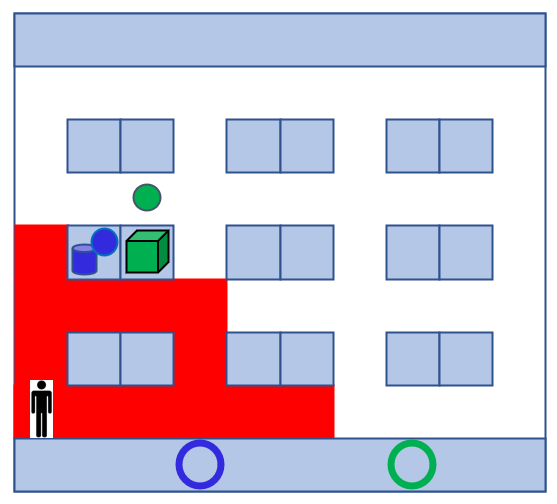
\includegraphics[scale=0.35]{figures/HITL1_case2_a.png}
    \caption{ケース2\ 状態$a$}
    \label{fig:HITL1_case2_a}
\end{figure}

\begin{figure}[!t]
    \centering
    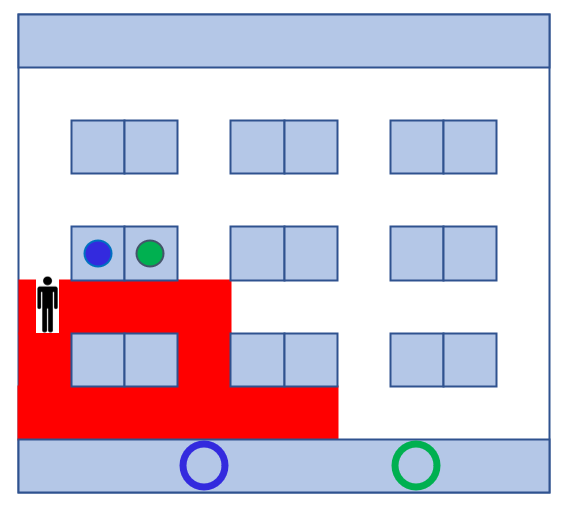
\includegraphics[scale=0.35]{figures/HITL1_case2_b.png}
    \caption{ケース2\ 状態$b$}
    \label{fig:HITL1_case2_b}
\end{figure}

図\ref{fig:HITL1_case2_b}のとき(協調作業が完了した後),人間がもとの作業場所に戻っていく.ロボット1,2は遷移先が人間の経路で進入禁止エリアになっているので,人間のゴール地点で安全が確認されるまで遷移は禁止される.

$H$が受理状態で自己ループする事象が生起したなら,スーパーバイザはロボット同士の衝突を回避する制御のみを行うようになる(図\ref{fig:HITL2_case2_c})

%人間は行動102により右に行くか,行動104により下に行くか2通りの遷移を持っている.102が生起したとき,ロボット1は人間が状態143に到達するまで遷移を禁止され,ロボット2は人間が状態144に遷移するまで行動を禁止される.一方,104が生起した場合,状態42,43が人間の経路から除外されることにより,ロボットの進入禁止エリアは図\ref{fig:human_area_3}のようになる.そのため,ロボット1,2ともに下に遷移することが可能になる. 

\begin{figure}[!t]
    \centering
    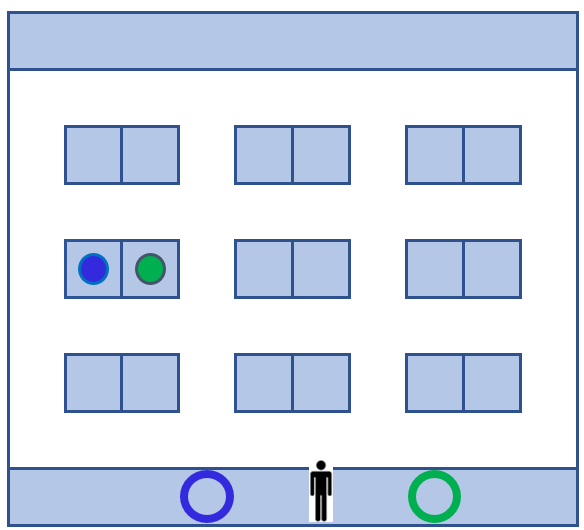
\includegraphics[scale=0.33]{figures/HITL1_case2_c.png}
    \caption{ケース2\ 状態$c$}
    \label{fig:HITL2_case2_c}
\end{figure}


\subsection{方法2}

ケース2でも,最小安全隔離距離は1マスとして,シミュレーションを行う.
先ほどと同じ例を用いて,動的に進入禁止エリアが変化する方法2での制御を考える.
この人間とロボットが協調する例を方法2で考えるとき,注意しなければならない点がある.
ロボット1に割り当てられた荷物の位置にロボットが存在し,協調作業場所(この例では隣のマス)に人間が存在しているときのみ,協調作業が可能である.また,タスクを完遂するには協調作業をするために,人間と人間の協力を必要とするロボット1が,荷物の積み込みをする際に近づかないといけないのである.
%ロボットの隣のマスに人間が存在しているタイミングで協調作業しなければならない.よって,
方法2の制御要求は,mutexという関数を用いて,同時に存在してほしくないロボットの状態と人間の状態の組み合わせを入力し,それらの状態の組を排除する制御要求を与えてスーパーバイザを作成する方法であった.
%ロボットと人間が一定の距離以上近づく事象を禁止するという制御要求がスーパーバイザに与えられる.
この例では,人間とロボットの間に1マス以上の間隔をあける制御要求があるので,スーパーバイザを計算する際に与える制御要求について,人間がロボット1を手伝う作業場所に存在し,ロボット1が目的の商品の場所にいる状態の組みを削除したものを制御要求として与える必要がある.
% この問題を解決しない限り,受理状態に到達するができない.
% 厳密にいえば,人間に接近するロボットの動作だけを禁止するわけではなく,

% つまり,ロボットが商品の場所で荷積みされるのを待っている状態のときその周りを人間が通れなくなってしまう.

しかし,このように制御要求のmutexに与える条件から1組だけ除くだけでは不十分であり,ブロッキング状態に陥る可能性がある.

次に,ブロッキング状態になる可能性がある問題の場面を,ケース2の例とは別の例を用いて紹介する.

図\ref{fig:HITL2_case2_d}のように,人間の助けを必要とするロボットが商品の棚の位置に,その隣に位置する協調作業場所に人間が向かっている場面を想定する.
このとき,人間は協調作業場所へ向かうために左に移動しなければならない.しかし,左に遷移してしまうことで,ロボットと人間が接近しないという制御要求を満たさなくなる.そのため,スーパーバイザに人間が左に遷移する行動を禁止されてしまう.
その結果,ロボットも人間も動くことができずブロッキング状態になる.
人間がそこに行って荷物を積まないと受理状態まで到達できないということで図\ref{fig:HITL2_case2_d}の状態になる前に,ロボットが棚に移動する動作をスーパーバイザが禁止する制御をする.

\begin{figure}[!t]
    \centering
    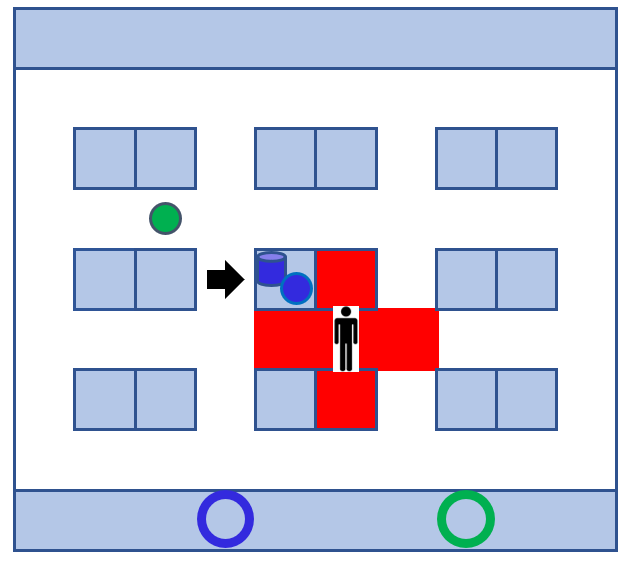
\includegraphics[scale=0.3]{figures/HITL2_case2_d.png}
    \caption{ケース2\ 状態$d$}
    \label{fig:HITL2_case2_d}
\end{figure}

%JIS規格によって,移載が安全に確実に行われるよう,インタロック機能の搭載が義務付けられているので,ロボットを荷物の棚の位置で待機させておくのが望ましいと考えられる.このような理由で,上記のスーパーバイザの制御は理想的でない.

また,その逆に人間が協調作業場所で待機しており,図\ref{fig:HITL2_case2_e}のように,ロボットが人間の周りのマスを経由して荷物の場所に向かっている場合についても同じ問題が生じる.ロボットの右に行く行動が禁止されてブロッキング状態になり,それを回避するため,スーパーバイザは人間が協調作業場所に到着する以前に制御を行うことになる.これは人間の行動を便宜上制御可能であると定義したことによって起こった問題である.

\begin{figure}[!t]
    \centering
    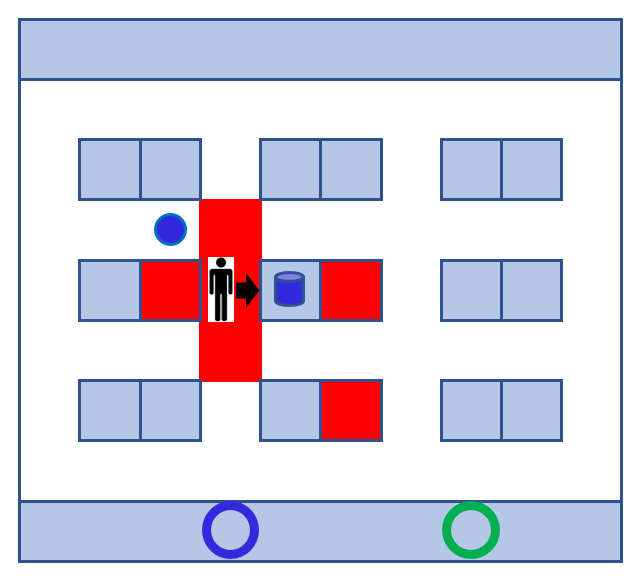
\includegraphics[scale=0.3]{figures/HITL2_case2_e.png}
    \caption{ケース2\ 状態$e$}
    \label{fig:HITL2_case2_e}
\end{figure}

これらを踏まえると,ロボットと人間が協力して積まれる荷物周辺では,制御要求を緩和して,ロボットと人間の接近を許可する制御が求められる.
つまり,協調して積み込む商品の保管場所近くでは,人間とロボットの間に距離をおくという制御要求の一部を削除する方法を提案する.
具体的には,mutexの条件のうち,ロボットが商品の場所に存在している状態を含むペアを削除し,次に人間が協調作業場所に存在している状態を含むペアを削除するといった2つの手順を踏んで考える.

%mutex(G, H, [s_G, s_H])と書き,Gが状態s_Gに,Hが状態s_Hに同時に存在する状態を排除することを意味する.状態のペア[s,s]を条件といい,%

まずは,前者のロボット1が商品を保管する棚である状態$[s_{G,item}]$にいるときの状態の組を除外する.
これはロボットが人間より先に協調作業場所に到着したときを想定した対策である(図\ref{fig:HITL2_case2_robot_waits_human}).

\begin{figure}[!t]
    \centering
    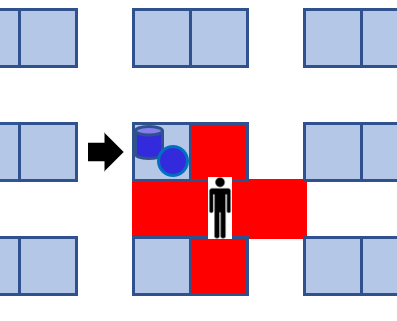
\includegraphics[scale=0.3]{figures/HITL2_case2_robot_waits_human.png}
    \caption{ロボットが待機しているときに発生し得るブロッキング状態}
    \label{fig:HITL2_case2_robot_waits_human}
\end{figure}

%mutexの条件のうち,ロボット側の状態にロボットに割り当てられた商品がある棚の状態が含まれているペアを,1組を除き削除する.削除の対象とならない状態のペアは,ロボットと人間が同じ状態に存在するペアである.

今回のシミュレーションでは,最小安全隔離距離を1マスとおいているので,人間側の状態に該当の位置の周りが含まれた状態のペアだけを削除すればよい.

%$G_1$が割り当てられた商品を保管する棚の状態が条件となっているペアを1組だけ除いて削除する.
商品のある棚の状態を$s_{G,item}$とすると,削除の対象となるのは$[s_{G,item},s_{G,item}-10], [s_{G,item},s_{G,item}-1], [s_{G,item},s_{G,item}+1], [s_{G,item},s_{G,item}+10]$である.
$[s_{G,item},s_{G,item}]$も状態$s_{G,item}$を含んでいる.しかし,ロボットと人間が同じ状態に存在する状態のペア$[s_{G,item},s_{G,item}]$は衝突回避の制御をする上で必要であるから,削除してはいけない.

もし,人間の安全を確保するために2マス以上確保しなければならないという制御要求を与えられていたなら,ロボット1が目的の商品の棚にいるときを含み,$G$と$H$が異なった状態にいるペアを削除することで解決される.

そして後者,人間が待機しているときロボットの経路に人間の周りが含まれていた場合も(図\ref{fig:HITL2_case2_human_waits_robot}),前者同様に,ロボットと人間の状態が同じペアを除いて,人間が協調作業場所にいるすべての状態のペアをmutexの条件から削除する.
%$[s_{H,help}-10,s_{H,help}], [s_{H,help}-1,s_{H,help}], [s_{H,help}+1,s_{H,help}], [s_{H,help}+10,s_{H,help}]$

\begin{figure}[!t]
    \centering
    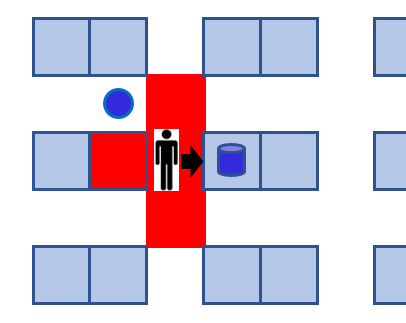
\includegraphics[scale=0.3]{figures/HITL2_case2_human_waits_robot.png}
    \caption{人間が待機しているときに発生し得るブロッキング状態}
    \label{fig:HITL2_case2_human_waits_robot}
\end{figure}

シミュレーションの結果である制御について解説する.

\begin{figure}[!t]
    \centering
    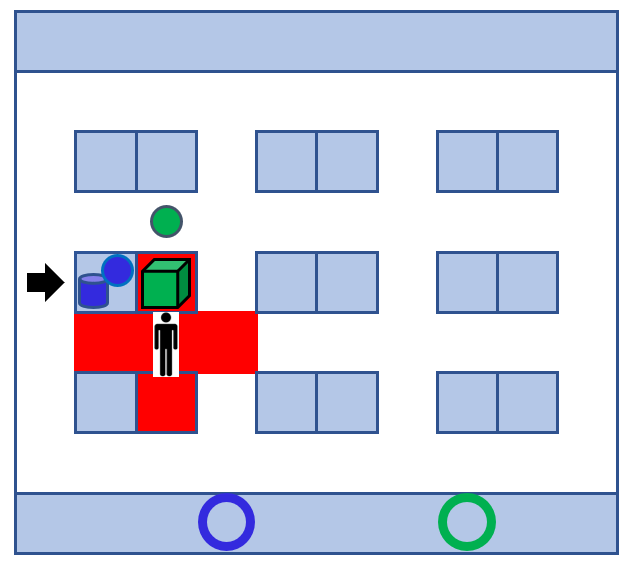
\includegraphics[scale=0.3]{figures/HITL2_case2_f.png}
    \caption{ケース2\ 状態$f$}
    \label{fig:HITL2_case2_f}
\end{figure}
\begin{figure}[!t]
    \centering
    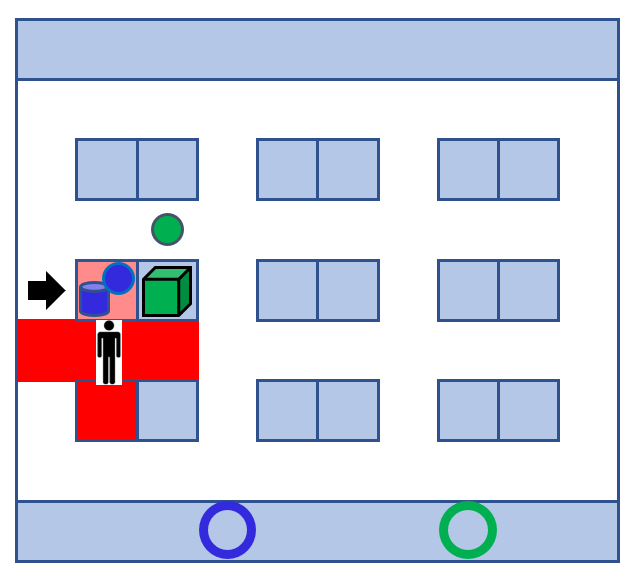
\includegraphics[scale=0.3]{figures/HITL2_case2_g.png}
    \caption{ケース2\ 状態$g$}
    \label{fig:HITL2_case2_g}
\end{figure}

図\ref{fig:HITL2_case2_f}の状態のとき,ロボット1は荷物のある状態32に待機しており,ロボット2は状態23に,人間が状態43に存在している.このとき,人間に荷物を積んでもらうまでロボット1の次に発生する行動は禁止され続ける.ロボット2の遷移先は,人間が近くにいるため進入禁止エリアとされているので,ロボット2の行動25が禁止される.また,$H$がとる可能性があるのは行動107である.ここで,ロボット1と人間に関する制御要求を緩和していることにより,人間の左へ遷移する行動が許されている.人間が左へ遷移したときの進入禁止エリアの変化は図\ref{fig:HITL2_case2_g}のようになる.図\ref{fig:HITL2_case2_g}の色の薄い進入禁止エリアはロボット2だけが対象であり,ロボット1には影響しない.

また,人間が協調作業場所に存在するとき,進入禁止エリアは図\ref{fig:HITL2_case2_h}のように変化する.

\begin{figure}[!t]
    \centering
    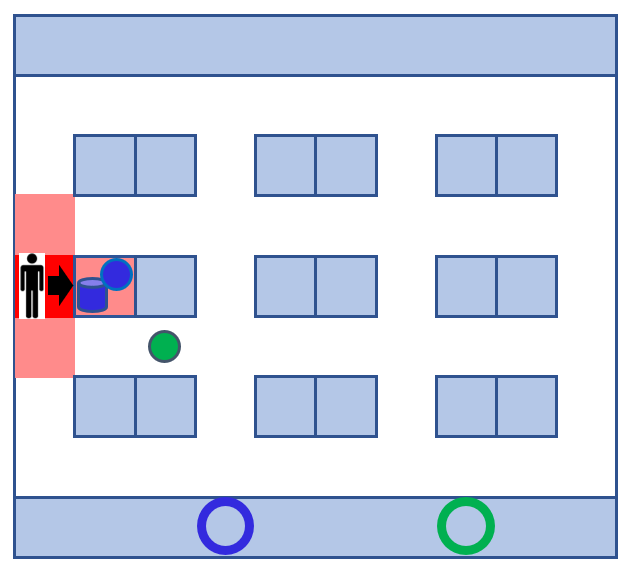
\includegraphics[scale=0.3]{figures/HITL2_case2_h.png}
    \caption{ケース2\ 状態$h$}
    \label{fig:HITL2_case2_h}
\end{figure}

商品の積み込みの作業が終わり,人間が移動すると,再びロボット1,2は人間のまわりに接近を禁止されるようになる(図\ref{fig:HITL2_case2_i}).

\begin{figure}[t]
    \centering
    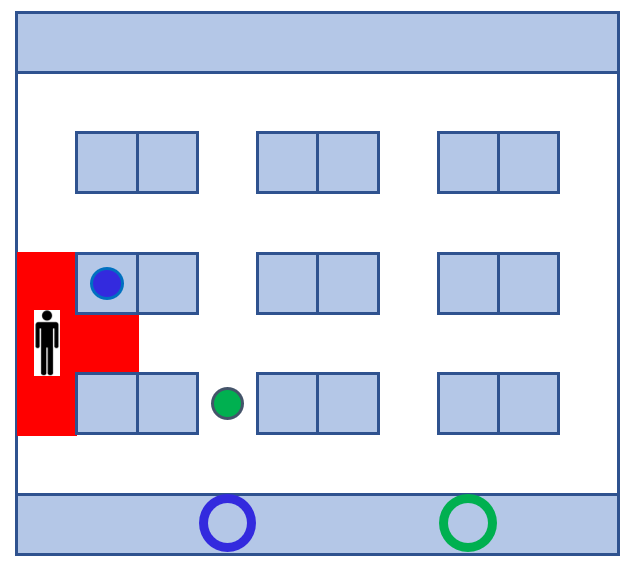
\includegraphics[scale=0.3]{figures/HITL2_case2_i.png}
    \caption{ケース2\ 状態$i$}
    \label{fig:HITL2_case2_i}
\end{figure}


\section{2つの方法の比較}
方法1としてロボットに人間の経路上を使用させない方法,方法2としてロボットを人間に決められた距離より接近させない方法の2つの制御方法によるケーススタディを紹介した.

方法1では,人間の経路に指定されていれば,人間が離れていてもロボットが使用できず,別のルートを通るか待つ必要があった.方法2をもちいると,離れているときは,ロボットが待つことなく走行ができるというメリットがある.

しかし,方法2は方法1に比べて,経路が増加するたびに計算時間も増加する傾向がある(表\ref{tb:run_time}).また,最小安全隔離距離の$d$が増えるにつれ,さらに計算量が増加してしまう.

比較の表について,制御要求を作成して,スーパーバイザの計算が終わるまでの計算時間の50回の平均を示している.また,$G_2$と$H$の状態遷移をそれぞれ経路の分岐が1つ増えるよう図\ref{fig:run_time_G2},\ref{fig:run_time_H}のように変更した.

\begin{table}[htb]
  \begin{tabular}{|l|r|r|r|r|} \hline
    &\ref{sect:case1}節の例 & $G_2$に遷移を追加 & $H$に遷移を追加 & $G_2$と$H$に遷移を追加 \\ \hline
    方法1 & 3.069 & 3.337 & 3.204 & 3.950 \\ \hline
    方法2 & 3.222 & 3.974 & 4.105 & 5.098 \\ \hline
  \end{tabular}
  \caption{計算時間の比較(単位 : 秒)}
  \label{tb:run_time}
\end{table}

\begin{figure}[h]
    \centering
    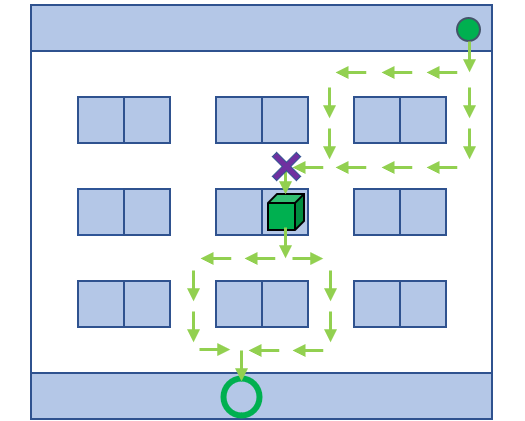
\includegraphics[scale=0.35]{figures/run_time_G2.png}
    \caption{変更後の$G_2$の経路}
    \label{fig:run_time_G2}
\end{figure}

\begin{figure}[h]
    \centering
    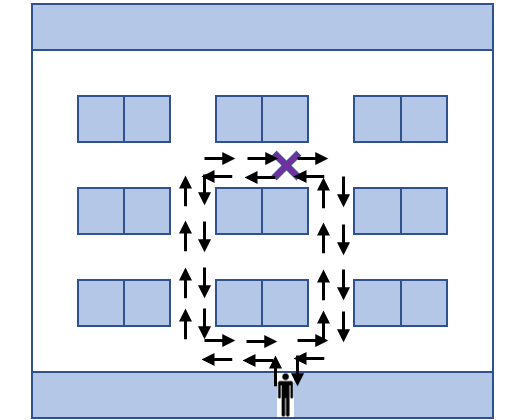
\includegraphics[scale=0.35]{figures/run_time_H.png}
    \caption{変更後の$H$の経路}
    \label{fig:run_time_H}
\end{figure}